\documentclass{article}

\usepackage[preprint]{neurips_2025}

\usepackage[utf8]{inputenc}
\usepackage[T1]{fontenc}
\usepackage{hyperref}
\usepackage{url}
\usepackage{booktabs}
\usepackage{amsfonts}
\usepackage{amsmath}
\usepackage{nicefrac}
\usepackage{microtype}
\usepackage{graphicx}
\usepackage{xcolor}
\usepackage{multirow}

% AUTO-GENERATED by scripts/make_paper_assets.py -- do not edit by hand.
\newcommand{\NumMatches}{10}
\newcommand{\NumTrainMatches}{6}
\newcommand{\NumValMatches}{2}
\newcommand{\NumTestMatches}{2}
\newcommand{\NumSeeds}{3}
\newcommand{\SeedList}{7, 11, 23}
\newcommand{\FalsConditionCount}{12}
\newcommand{\PredictionGapSeconds}{1.0}
\newcommand{\FpsOut}{10}
\newcommand{\FeatureCount}{7}
\newcommand{\NumWindows}{315,400}
\newcommand{\NumTdExamples}{178,344}
\newcommand{\ZDim}{128}
\newcommand{\NumLayers}{2}
\newcommand{\NumHeads}{4}
\newcommand{\EmaMomentum}{0.996}
\newcommand{\VarianceThreshold}{0.05}
\newcommand{\SlotReconWeight}{0.25}
\newcommand{\ContextReconWeight}{0.05}
\newcommand{\MarginWeight}{0.1}
\newcommand{\MarginValue}{0.01}
\newcommand{\BatchSize}{128}
\newcommand{\LearningRate}{0.001}
\newcommand{\VariantCount}{8}
\newcommand{\TorchVersion}{2.12.1}
\newcommand{\NumTestsPassed}{181}
\newcommand{\DiscoveryFamilyCount}{5}
\newcommand{\PanelPositiveRows}{20}
\newcommand{\PanelControlRows}{20}
\newcommand{\GateOverallStatus}{blocked}
\newcommand{\ProbeTotalContrasts}{6}
\newcommand{\ProbeBlockedContrasts}{3}
\newcommand{\PanelAnnotatorCount}{5}
\newcommand{\PanelFleissKappa}{0.33}
\newcommand{\PanelHeadline}{inter-model agreement of Fleiss' $\kappa$ = 0.33 and a majority-vote enrichment of -0.42 positive-label rate over hidden controls (Fisher $p$ = 1.000)}
\newcommand{\PanelCompletionNote}{5 of 5 attempted annotators completed all items (Codex (GPT-5.5), Fable, Kimi, Opus, Sonnet).}
\newcommand{\PanelMajorityFisher}{1.000}
\newcommand{\PanelMajorityRisk}{-0.42}
\newcommand{\FalsStatus}{controls\_passed}
\newcommand{\FalsWrongMatchMeanRatio}{5.00}
\newcommand{\FalsShuffledMeanRatio}{4.96}
\newcommand{\FalsNoMotionMeanRatio}{2.27}
\newcommand{\FalsNoMotionMinRatio}{1.81}
\newcommand{\FalsTeamLabelSwapMeanRatio}{3.17}
\newcommand{\FalsTargetTeamLabelSwapMeanRatio}{11.28}
\newcommand{\FalsSlotPermMinRatio}{1.29}
\newcommand{\FalsTeamSwapMeanRatio}{3.31}
\newcommand{\FalsReversedTimeMeanRatio}{1.03}
\newcommand{\FalsMaskedBallMeanRatio}{1.09}
\newcommand{\FalsPassRatio}{1.25}
\newcommand{\FalsCautionRatio}{1.05}
\newcommand{\FalsTestStatus}{controls\_passed}
\newcommand{\FalsTestScopeClause}{on both the validation matches used for candidate selection and the held-out test matches}
\newcommand{\AblationOutcome}{Without reconstruction, the latents do not collapse (mean per-dimension std 0.325, min 0.090), so anti-collapse is carried by the EMA asymmetry and margin term rather than by reconstruction. The temporal side of the battery \emph{strengthens}: shuffled futures hurt 7.59$\times$, wrong-match futures 7.53$\times$, the no-motion identity loses by 48.37$\times$, and even reversed-time sensitivity rises to 1.18$\times$. But the identity side collapses: player-slot permutation (1.00$\times$) and team-slot swap (1.00$\times$) barely move the loss, so the ablated model would be blocked by the battery's identity controls. The hybrid's reconstruction heads are therefore load-bearing not for anti-collapse but for identity sensitivity --- and they buy it at the price of temporal directedness, which mechanistically explains the configuration-over-dynamics character of the passing candidate. }
\newcommand{\ProbeDisplRawMean}{+0.070}
\newcommand{\ProbeDisplZMean}{+0.241}
\newcommand{\ProbeShapeZMean}{+0.049}
\newcommand{\ProbeShapeRawMean}{-0.031}
\newcommand{\ProbeGlobalXRawMin}{-0.006}
\newcommand{\ProbeGlobalXRawMean}{+0.002}
\newcommand{\ProbeGlobalXZMean}{-0.016}
\newcommand{\ProbeGlobalXRawSeedMax}{+0.013}
\newcommand{\DiscEntropyLatent}{0.847}
\newcommand{\DiscEntropyBestControl}{0.866}
\newcommand{\DiscEntropyMargin}{-0.019}
\newcommand{\DiscTopMatchLatent}{0.550}
\newcommand{\DiscTopMatchBestControl}{0.490}
\newcommand{\DiscTopMatchMargin}{-0.059}
\newcommand{\DiscMinHeldout}{0}
\newcommand{\DiscMagTopFraction}{1.00}
\newcommand{\DiscTopMatchLatentMin}{0.230}
\newcommand{\DiscTopMatchLatentMax}{1.000}
\newcommand{\GateBlockingGates}{probe\_incremental, discovery\_controls, blinded\_annotation}
\providecommand{\FalsificationNarrative}{\textit{[results pending]}}
\providecommand{\ProbeNarrative}{\textit{[results pending]}}
\providecommand{\DiscoveryNarrative}{\textit{[results pending]}}
\providecommand{\GateNarrative}{\textit{[results pending]}}
\providecommand{\CleanroomNarrative}{\textit{[results pending]}}
\providecommand{\PanelNarrative}{\textit{[results pending]}}


\title{Gates Before Claims: A Leakage-Controlled Evaluation Protocol for
Self-Supervised Representations of Soccer Tracking Data}

\author{%
  Luis Lozano \\
  Tecnol\'ogico de Monterrey \\
  \texttt{lalozanom@gmail.com} \\
  \And
  Emilio Calder\'on \\
  University of California, Berkeley \\
}

\begin{document}

\maketitle

\begin{abstract}
Self-supervised representations of multi-agent sports tracking data invite
over-interpretation: latent clusters become ``tactics,'' prediction residuals
become ``tactical surprise,'' and probe accuracy on leaked channels becomes
``emergent understanding.'' We present an integrity-gated evaluation protocol
that makes such claims mechanically expensive. The protocol combines immutable
hashed match splits, leakage-controlled feature views, a non-overlapping
future-prediction objective, a \FalsConditionCount-condition falsification
battery, incremental-value probes that compare raw kinematics against
raw-plus-latent features at seed and match level, discovery controls that pit
latent transition clusters against raw, PCA, random-encoder, and handcrafted
baselines, blinded annotation with hidden matched controls, and a
machine-readable claim gate that emits explicit blocking conditions. As a case
study, we train a temporal-difference joint-embedding predictive architecture
(TD-JEPA) on \NumMatches{} broadcast-tracking matches and run it through every
gate. The candidate representation passes the falsification battery across
\NumSeeds{} seeds but records negative incremental value on
\ProbeBlockedContrasts{} of \ProbeTotalContrasts{} probe contrasts and does not
separate from control baselines in discovery, so the protocol's verdict is
\emph{\GateOverallStatus}: no tactical claim is licensed. An independent
clean-room reproduction on a second machine, from public data to final gate,
reproduces the qualitative gate outcome. A blinded panel of
\PanelAnnotatorCount{} frontier-model annotators, used as a diagnostic in place
of not-yet-available human annotation, shows \PanelHeadline. We release the
protocol, gate tooling, and all run manifests; we argue that negative results
under honest gates are the correct default deliverable for small-data sports
representation learning.
\end{abstract}

\section{Introduction}
\label{sec:intro}

Optical and broadcast tracking now yields dense multi-agent time series for
every professional soccer match: 22 player trajectories plus the ball, sampled
at 10--25\,Hz. A natural research program is to learn self-supervised
representations of these trajectories and then interpret the learned latent
space --- its clusters as tactical motifs, its prediction residuals as
surprising moments, its probe performance as evidence of emergent game
understanding. Versions of this program appear across sports analytics,
from formation discovery~\citep{bialkowski2014large} and tactic
mining~\citep{decroos2018tactics} to trajectory
generation~\citep{le2017coordinated,yeh2019diverse,zhan2019generating} and
multi-entity transformers~\citep{alcorn2021baller2vec}.

The failure modes of this program are equally well documented, just usually in
other fields. Leakage inflates evaluations~\citep{kapoor2023leakage};
overlapping windows masquerade as independent samples~\citep{lones2021pitfalls};
benchmark variance swallows claimed improvements~\citep{bouthillier2021accounting};
and clustering algorithms will happily partition any point
cloud~\citep{rousseeuw1987silhouettes}, tactical or not. Sports tracking data
aggravates all four: matches are few, frames within a match are strongly
autocorrelated, provider metadata (possession flags, visibility masks) leaks
label information into inputs, and smooth kinematics dominate any
distance-based structure.

This paper takes the position that for small-data sports representation
learning, the evaluation protocol --- not the representation --- should be the
primary contribution, and the protocol should be built to \emph{block} claims
by default. We describe such a protocol, implemented end-to-end in a working
codebase, and report what happens when a reasonable self-supervised candidate
is pushed through it.

Concretely, we make four contributions:

\begin{enumerate}
  \item \textbf{An integrity-gated evaluation protocol} for self-supervised
  tracking representations (Section~\ref{sec:protocol}): immutable hashed
  inductive match splits; leakage-controlled feature views; a non-overlapping
  future-prediction objective; a \FalsConditionCount-condition falsification
  battery; incremental-value probes reported at seed and match level; discovery
  controls against raw, PCA, random-encoder, and handcrafted baselines; blinded
  annotation with hidden matched controls; and a combined machine-readable gate
  that names each blocking condition.
  \item \textbf{A negative/mixed case study} (Sections~\ref{sec:setup} and
  \ref{sec:results}): a TD-JEPA representation trained on \NumMatches{} public
  broadcast-tracking matches~\citep{skillcorner2020opendata} that passes
  falsification across \NumSeeds{} seeds yet fails the incremental-value and
  discovery gates, yielding an overall claim status of \emph{\GateOverallStatus}.
  \item \textbf{An independent clean-room reproduction} (Section~\ref{sec:cleanroom}):
  a second author re-executed the full pipeline --- public data download, split
  verification, training, and all gates --- on different hardware and software
  versions, reproducing the qualitative gate outcomes. Following
  \citet{raff2019reproducibility}, we treat independent re-execution, not
  artifact re-loading, as the reproducibility standard.
  \item \textbf{A blinded model-annotator panel} (Section~\ref{sec:panel}): with
  human annotation still pending, \PanelAnnotatorCount{} frontier models
  independently annotated a balanced blinded package of high-residual clips and
  hidden matched controls under a controlled label vocabulary. We report
  agreement (Fleiss' $\kappa$~\citep{fleiss1971measuring}, pairwise Cohen's
  $\kappa$~\citep{cohen1960coefficient}) and enrichment against the hidden
  controls, and we are explicit that this panel is a diagnostic, not a
  substitute for the human gate.
\end{enumerate}

We frame the outcome plainly. The candidate representation is a competent
engineering baseline: it trains stably, its embeddings do not collapse, and it
beats shuffled- and wrong-match falsification controls. But under gates that
price in leakage, autocorrelation, and control baselines, it has not earned a
single tactical claim. We think this is the right default outcome to
publish for this regime, and the protocol makes it cheap to publish honestly.

\section{Related Work}
\label{sec:related}

\paragraph{Joint-embedding predictive architectures.}
JEPA-style models predict target representations from context representations
rather than reconstructing inputs~\citep{lecun2022path,assran2023ijepa,bardes2024vjepa}.
Our candidate follows this family: an EMA target
encoder~\citep{grill2020byol}, a predictor over latent states, and a variance
regularizer~\citep{bardes2022vicreg} to resist collapse~\citep{chen2021simsiam}.
Sports tracking is an attractive JEPA domain --- agents are few, dynamics are
smooth, semantics are contested --- but exactly that smoothness makes trivial
temporal interpolation a competitive predictor, which motivates our
non-overlap objective and no-motion margin controls.

\paragraph{Soccer tracking analytics.}
Prior work spans formation and role discovery~\citep{bialkowski2014large,shaw2019dynamic},
tactic pattern mining~\citep{decroos2018tactics}, action
valuation~\citep{decroos2019actions,fernandez2018wide,spearman2018beyond},
ghosting and trajectory generation~\citep{le2017coordinated,yeh2019diverse,zhan2019generating},
and multi-agent trajectory prediction more broadly~\citep{alahi2016social,alcorn2021baller2vec}.
Much of this literature validates discovered structure by expert inspection of
selected examples. Our protocol replaces selected examples with blinded,
control-matched annotation, and replaces single-run clustering with
multi-seed, multi-family control comparisons.

\paragraph{Leakage, variance, and reproducibility.}
Our gate design operationalizes, for one domain, the general warnings of
\citet{kapoor2023leakage} on leakage, \citet{lones2021pitfalls} on temporal
data hygiene, \citet{bouthillier2021accounting} and \citet{henderson2018deep}
on variance-aware comparison, \citet{musgrave2020metric} on inflated
metric-learning claims, \citet{dodge2019show} and \citet{pineau2021improving}
on reporting standards, and \citet{simmons2011false} on researcher degrees of
freedom. The clean-room reproduction follows \citet{raff2019reproducibility}
in privileging independent re-execution. Our contribution is not new theory
but a working, machine-checkable instantiation for tracking data, where the
autocorrelation and metadata-leakage traps are unusually severe.

\section{The Integrity Protocol}
\label{sec:protocol}

The protocol is a chain of gates. Each gate consumes artifacts stamped with
provenance metadata and emits a machine-readable summary; a final aggregator
combines them into one claim status with named blocking conditions. Nothing
downstream of a failed gate may be interpreted as evidence. Figure~\ref{fig:pipeline}
summarizes the flow.

\begin{figure}[t]
  \centering
  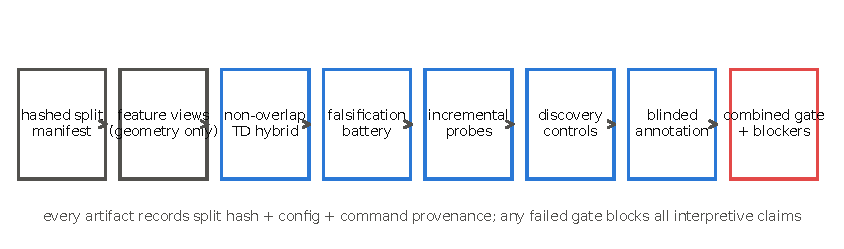
\includegraphics[width=\linewidth]{figures/pipeline.pdf}
  \caption{The integrity-gated evaluation pipeline. Every scientific artifact
  records the split-manifest hash, feature view, objective mode, and command
  provenance. The combined gate emits an overall claim status plus one named
  blocking condition per failure; downstream stages of a blocked gate are
  diagnostics by definition.}
  \label{fig:pipeline}
\end{figure}

\subsection{Split lineage and provenance}
\label{sec:protocol-splits}

All experiments inherit a single immutable split manifest: \NumMatches{}
matches partitioned inductively into \NumTrainMatches{} training,
\NumValMatches{} validation, and \NumTestMatches{} test matches. The manifest
is hashed (SHA-256 over a canonical JSON serialization), and every downstream
artifact --- window tensors, TD datasets, checkpoints, embeddings, probe
datasets, transition datasets, cluster summaries --- stores the hash it was
built from. Loaders reject artifacts whose hashes disagree, dataset names
outside an allow-list, and scientific runs that lack period-aware sample
identities (\texttt{match\_id:period:frame}), which prevents cross-period
frame-index collisions from silently corrupting alignment. Each entry point
writes a run manifest recording the git commit, config hash, split hash,
feature view, objective mode, and platform. Distinct match halves and a
prediction-gap exclusion ensure that no training window overlaps an
evaluation window.

\subsection{Leakage-controlled feature views}
\label{sec:protocol-views}

Tracking providers ship metadata channels --- possession flags, visibility
masks --- that trivially predict several popular probe targets. The protocol
defines explicit feature views: \texttt{full\_state\_legacy} (all channels;
allowed only as an engineering baseline), \texttt{geometry\_only} (positions
and velocities; the scientific view), \texttt{missingness\_only\_control}, and
\texttt{raw\_kinematics\_control}. Probes are classified by validity:
possession-related probes on full-state embeddings are labeled leakage sanity
checks and can never support semantic claims.

\subsection{Non-overlap objective and falsification battery}
\label{sec:protocol-falsification}

The legacy TD objective predicts $z_{t+\Delta}$ from a context window that
overlaps the target frames; smooth kinematics make this nearly free.
The scientific objective, \texttt{future\_nonoverlap\_context\_only},
enforces a temporal gap of \PredictionGapSeconds{}s between context and
target, with a margin term requiring the predictor to beat the no-motion
(identity) latent. A trained checkpoint then faces \FalsConditionCount{}
falsification conditions, including shuffled futures within batch, futures
from another match, reversed-time context, masked ball, team-slot and
home/away label swaps on context and target sides, pitch reflection, and
consistent player-slot permutations. Passing requires the correct pairing to
beat corrupted pairings by a ratio threshold on the gated loss, consistently
across seeds; near-invariance to any semantically meaningful corruption is a
named blocker.

\subsection{Incremental-value probes}
\label{sec:protocol-probes}

A representation $z$ earns probe credit only through \emph{incremental} value:
for each held-out target we train identical probes on raw kinematic summaries,
on $z$, on raw$+z$, and on shape-matched random features, and report
$\mathrm{perf}(\mathrm{raw}{+}z) - \mathrm{perf}(\mathrm{raw})$ with sign
conventions fixed per metric. Increments are aggregated across \NumSeeds{}
encoder seeds and, crucially, across held-out matches: a contrast blocks if
its increment is non-positive in the mean or negative for any seed or any
held-out match. Global-$x$ displacement targets are labeled geometry, not
``attacking progression''; team-shape targets are labeled all-visible-player
diagnostics.

\subsection{Discovery controls}
\label{sec:protocol-discovery}

Latent transition clustering (k-means over $\Delta z$ with train-fit,
held-out-assign protocol) is compared against \DiscoveryFamilyCount{} control
feature families: raw coordinate/velocity transitions, PCA of raw transitions,
random-encoder deltas, and handcrafted structure-change metrics (raw and PCA
variants), each clustered across the same seeds. The latent family must
separate from the best control by a margin on cluster-size entropy and on
top-match concentration, avoid sparse held-out clusters, and avoid
transition-magnitude domination. Without separation, clusters are partitions
of smooth motion, not discovered structure.

\subsection{Blinded annotation with hidden controls}
\label{sec:protocol-annotation}

Only after the quantitative gates does the protocol permit visualization, and
then only blinded: a balanced package of \PanelPositiveRows{} high-residual
clips and \PanelControlRows{} magnitude-matched low-residual controls is
rendered with all identifying fields (cluster id, residual score,
positive/control status) moved to a private key file. Annotators see a fixed
label vocabulary (\texttt{tactical\_pattern}, \texttt{routine\_motion},
\texttt{tracking\_artifact}, \texttt{ambiguous}); the analyzer rejects any
other label, reports enrichment of positive labels in the high-residual group
against the hidden controls (risk difference and Fisher exact test), and
refuses to upgrade any claim while the package is incomplete.

\subsection{The combined gate}
\label{sec:protocol-gate}

A final aggregator merges the falsification, probe, discovery, and annotation
summaries into one artifact with an overall claim status
(\texttt{supported\_for\_further\_validation} at best, \texttt{blocked}
otherwise), the list of named blocking conditions, and a suggested next
scientific action. The gate is deliberately asymmetric: one failed gate blocks
all interpretive claims, while passing everything licenses only ``supported
for further validation,'' never a tactical conclusion by itself.

\section{Case Study Setup}
\label{sec:setup}

\paragraph{Data.}
We use the \NumMatches{} publicly released SkillCorner broadcast-tracking
matches~\citep{skillcorner2020opendata}, resampled to \FpsOut{}\,Hz, in a
canonical 23-entity representation (22 player slots plus ball) with
\FeatureCount{} geometry channels per entity under the scientific view. Raw
tracking for every match covers both halves; window preparation validates
per-period coverage against the raw files and refuses stale caches. The
combined evaluation window tensor contains \NumWindows{} windows
(2\,s context, 2\,s horizon, 0.2\,s stride). The TD dataset under the
non-overlap objective contains \NumTdExamples{} examples (1\,s context,
\PredictionGapSeconds{}s gap).

\paragraph{Model and training.}
The encoder is a compact spatiotemporal transformer~\citep{vaswani2017attention}
(\ZDim-dimensional latents, \NumLayers{} layers, \NumHeads{} heads) with an
EMA target encoder (momentum \EmaMomentum), a latent predictor, a variance
regularizer (threshold \VarianceThreshold), slot-aligned target and
context reconstruction heads (weights \SlotReconWeight{} and
\ContextReconWeight), and a no-motion margin term (weight \MarginWeight,
margin \MarginValue). We train with Adam~\citep{kingma2015adam} in
PyTorch~\citep{paszke2019pytorch}, batch size \BatchSize, learning rate
\LearningRate, for one epoch per seed --- the protocol's diagnostic budget ---
across seeds \SeedList. This candidate configuration was selected by the
first-stage falsification gate from \VariantCount{} objective variants
explored under the same protocol (longer gaps, CLS pooling, slot
reconstruction, margin, and context-reconstruction weights); all selection
used validation matches only.

\paragraph{Clean-room design.}
\label{par:cleanroom-design}
The pipeline was first executed by one author on his machine; a second
execution was then performed independently on different hardware (Apple
M3~Max, CPU-only) and different library versions (Python 3.13, PyTorch
\TorchVersion), starting from a fresh clone, a fresh public-data download, and
split-manifest verification, driven by a scripted runner committed to the
repository. We compare gate outcomes, not floating-point values, and report
both runs' blocking conditions in Section~\ref{sec:cleanroom}.

\section{Results}
\label{sec:results}

\subsection{Falsification battery}
\label{sec:results-falsification}

\begin{table}[t]
  \centering
  \small
  \begin{tabular}{lrrrl}
    \toprule
    Condition & Ratio mean & Ratio min & Ratio max & Status \\
    \midrule
    target team label swap & 11.278 & 10.624 & 12.076 & pass \\
    pitch reflection & 5.260 & 4.975 & 5.480 & pass \\
    future from another match & 4.999 & 4.726 & 5.284 & pass \\
    shuffled future within batch & 4.963 & 4.695 & 5.249 & pass \\
    team swap & 3.311 & 3.162 & 3.508 & pass \\
    team label swap & 3.166 & 3.043 & 3.318 & pass \\
    no motion predictor & 2.269 & 1.812 & 2.858 & pass \\
    consistent player slot permutation & 1.414 & 1.355 & 1.483 & pass \\
    target consistent player slot permutation & 1.355 & 1.292 & 1.450 & pass \\
    masked ball & 1.085 & 1.061 & 1.098 & caution \\
    reversed time context & 1.030 & 1.029 & 1.031 & fail \\
    \bottomrule
  \end{tabular}
  \caption{Falsification battery on validation matches, gated on total loss across seeds 7, 11, 23. Ratios are corrupted-condition loss over correct-pairing loss (higher means the corruption hurts, as it should); pass requires min ratio $\geq$ 1.25, caution $\geq$ 1.05. Reversed-time and masked-ball are reported but excluded from blocking by protocol. Overall: \textbf{controls\_passed}.}
  \label{tab:falsification}
\end{table}


Table~\ref{tab:falsification} and Figure~\ref{fig:falsification} report the
battery. The gate verdict is \emph{\FalsStatus}: every blockable corruption
raises the gated loss past the pass threshold of \FalsPassRatio$\times$ in all
\NumSeeds{} seeds. Futures drawn from another match
(\FalsWrongMatchMeanRatio$\times$) and shuffled futures
(\FalsShuffledMeanRatio$\times$) hurt most among pairing controls; team-identity
corruptions hurt $3$--$11\times$; and the learned predictor beats the no-motion
identity by \FalsNoMotionMeanRatio$\times$ on average (worst seed
\FalsNoMotionMinRatio$\times$) --- the margin term introduced during candidate
selection is doing its job. The slot-permutation controls, the sprint's
historical weak point, now clear the bar with worst-case
\FalsSlotPermMinRatio$\times$. Two excluded-from-blocking diagnostics remain
informative: reversed-time context (\FalsReversedTimeMeanRatio$\times$) and
masked ball (\FalsMaskedBallMeanRatio$\times$) barely move the loss, telling us
the representation leans on configuration far more than on arrow-of-time or
ball-specific signal at this horizon. Passing this battery licenses exactly
one claim: the encoder learned non-trivial temporal structure. Whether that
structure is \emph{useful} is the next gate's question.

\begin{figure}[t]
  \centering
  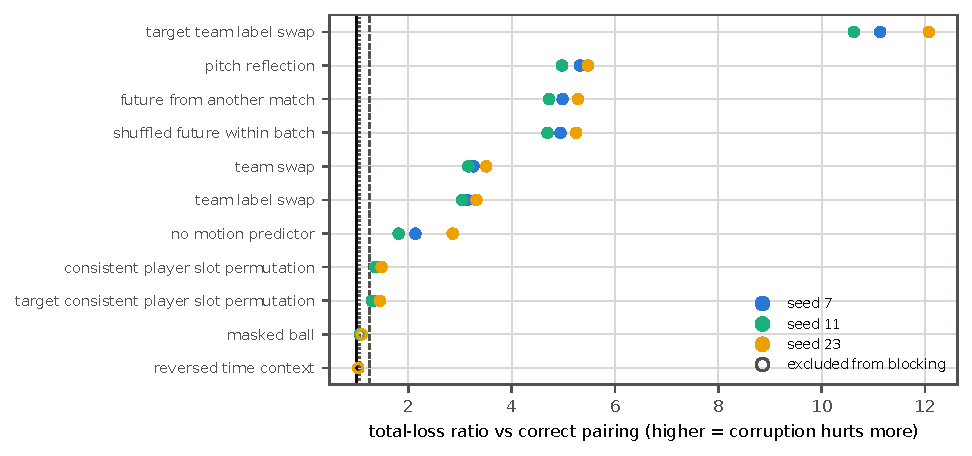
\includegraphics[width=0.9\linewidth]{figures/falsification.pdf}
  \caption{Falsification ratios per condition (one marker per seed; gated on
  total loss). Dashed line: pass threshold \FalsPassRatio; dotted: caution
  \FalsCautionRatio; open markers: conditions excluded from blocking by
  protocol.}
  \label{fig:falsification}
\end{figure}

\subsection{Incremental-value probes}
\label{sec:results-probes}

\begin{table}[t]
  \centering
  \small
  \begin{tabular}{llrrrrl}
    \toprule
    Target & Contrast & \multicolumn{2}{c}{Seed-level incr.} & \multicolumn{2}{c}{Match-level incr.} & Verdict \\
    & & mean & min & mean & min & \\
    \midrule
    future ball displacement m & raw$+z$ vs raw & 0.0699 & 0.0614 & 0.0707 & 0.0625 & \textcolor[HTML]{2a78d6}{positive} \\
    future ball displacement m & raw$+z$ vs raw (z-scored) & 0.2412 & 0.1951 & 0.2419 & 0.1956 & \textcolor[HTML]{2a78d6}{positive} \\
    future ball global x bucket & raw$+z$ vs raw & 0.0018 & -0.0060 & 0.0023 & -0.0054 & \textcolor[HTML]{e34948}{blocked} \\
    future ball global x bucket & raw$+z$ vs raw (z-scored) & -0.0163 & -0.0221 & -0.0164 & -0.0223 & \textcolor[HTML]{e34948}{blocked} \\
    team shape change bucket & raw$+z$ vs raw & -0.0310 & -0.0427 & -0.0310 & -0.0423 & \textcolor[HTML]{e34948}{blocked} \\
    team shape change bucket & raw$+z$ vs raw (z-scored) & 0.0486 & 0.0409 & 0.0476 & 0.0407 & \textcolor[HTML]{2a78d6}{positive} \\
    \bottomrule
  \end{tabular}
  \caption{Incremental value of $z$ over raw kinematics for linear probes on held-out matches. Signed improvement is oriented so positive is better regardless of metric direction. A contrast is blocked if any seed-level or match-level increment is non-positive; the gate records 3 of 6 contrasts as positive.}
  \label{tab:probes}
\end{table}


Table~\ref{tab:probes} and Figure~\ref{fig:probes} report incremental value.
The picture is mixed in a specific, instructive way. Where the target is
close to dynamics --- future ball displacement --- adding $z$ helps
consistently in every seed and every held-out match
(\ProbeDisplRawMean{} RMSE improvement on the raw view, \ProbeDisplZMean{}
z-scored). Team-shape change shows the same gain only under z-scoring
(\ProbeShapeZMean); on the unnormalized view, adding $z$ actively hurts
(\ProbeShapeRawMean). The global-$x$ bucket target fails both views: its raw
increment is positive on average (\ProbeGlobalXRawMean) but negative for at
least one seed (min \ProbeGlobalXRawMin), and z-scoring makes it reliably
negative (\ProbeGlobalXZMean). Under the gate's rule --- an increment must be
positive for \emph{every} seed and \emph{every} held-out match --- two of
three targets block. We highlight the global-$x$ case: judged on a single
seed (seed 7 gives $+0.013$), it would have passed; the three-seed minimum
reverses the conclusion. This is the concrete, small-data version of
variance-aware benchmarking~\citep{bouthillier2021accounting}, and it is why
the protocol refuses single-seed probe evidence.

\begin{figure}[t]
  \centering
  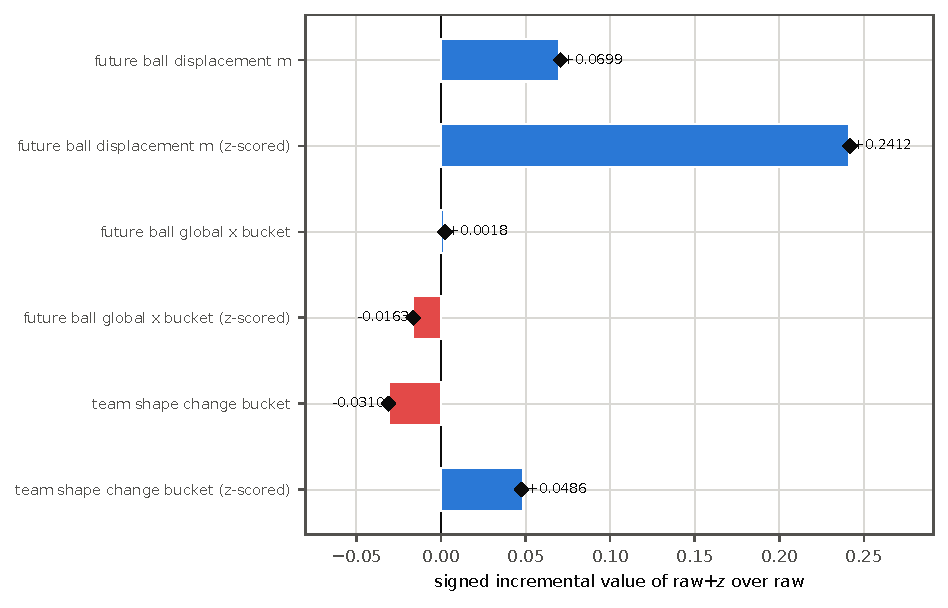
\includegraphics[width=0.88\linewidth]{figures/probes.pdf}
  \caption{Signed incremental value of raw$+z$ over raw per target and view
  (bars: mean across seeds; diamonds: match-level mean). Blue: positive;
  red: negative. The gate blocks any contrast with a non-positive seed-level
  or match-level increment.}
  \label{fig:probes}
\end{figure}

\subsection{Discovery controls}
\label{sec:results-discovery}

\begin{table}[t]
  \centering
  \small
  \begin{tabular}{lrr}
    \toprule
    Feature family & Cluster-size entropy $\uparrow$ & Top-match fraction $\downarrow$ \\
    \midrule
    TD-JEPA (normalized $\Delta z$) & 0.847 [0.834, 0.858] & 0.550 \\
    raw transitions & 0.857 [0.847, 0.869] & 0.516 \\
    PCA of raw transitions & 0.866 [0.864, 0.869] & 0.490 \\
    random-encoder $\Delta z$ & 0.845 [0.840, 0.850] & 0.520 \\
    handcrafted structure$^{\dagger}$ & 0.965 [0.960, 0.968] & 0.218 \\
    PCA of handcrafted structure$^{\dagger}$ & 0.969 [0.965, 0.973] & 0.221 \\
    \midrule
    margin vs best control & -0.019 & -0.059 \\
    \bottomrule
  \end{tabular}
  \caption{Discovery families at $k{=}32$, $\Delta{=}0.2$\,s: mean [min, max] over clustering seeds. The gate requires the latent family to beat the best of the raw/PCA/random controls by $+0.02$ on both metrics ($^{\dagger}$handcrafted families are required to be present but sit outside the margin's control set). Further latent blockers: min held-out examples per cluster 0; top-magnitude transition share in one cluster 1.00.}
  \label{tab:discovery}
\end{table}


\DiscoveryNarrative

\subsection{The combined gate}
\label{sec:results-gate}

\begin{table}[t]
  \centering
  \small
  \begin{tabular}{llp{7.4cm}}
    \toprule
    Gate & Status & Blocking conditions \\
    \midrule
    falsification & controls\_passed & none \\
    probe incremental & diagnostic\_only & 12 condition strings over \texttt{future\_ball\_global\_x\_bucket}, \texttt{team\_shape\_change\_bucket} \\
    discovery controls & diagnostic\_only & \texttt{latent\_entropy\_not\_separated\_from\_controls}, \texttt{latent\_match\_concentration\_not\_separated\_from\_controls}, \texttt{sparse\_heldout\_clusters}, \texttt{transition\_magnitude\_concentration} \\
    blinded annotation & diagnostic\_only & none \\
    \midrule
    \textbf{overall} & \textbf{blocked} & next action: Resolve mixed incremental probe results or redesign the representation before treating discovery or annotation as evidence. \\
    \bottomrule
  \end{tabular}
  \caption{The combined integrity gate. Any blocked sub-gate blocks all interpretive claims; the artifact also names the next scientific action.}
  \label{tab:gate}
\end{table}


\GateNarrative

\subsection{Clean-room reproduction}
\label{sec:cleanroom}

\begin{table}[t]
  \centering
  \small
  \begin{tabular}{lccc}
    \toprule
    Gate outcome & Original run & Clean-room run & Agreement \\
    \midrule
    falsification status & controls\_passed & controls\_passed & \textbf{agree} \\
    probe blocking targets & 2 & 2 (3 contrasts, 12 condition strings) & \textbf{agree} \\
    discovery blockers & 4 & 4 & \textbf{agree} \\
    overall claim status & blocked & blocked & \textbf{agree} \\
    \bottomrule
  \end{tabular}
  \caption{Clean-room re-execution: gate outcomes from the original run (original-run head \texttt{349fc08}, as recorded in the repository's integrity documentation committed at \texttt{acb2ba3}) versus this paper's second-operator re-execution on different hardware and library versions. We compare gate outcomes and named blockers, not floating-point losses. Blocker vocabulary: 2 blocking \emph{targets} = 3 blocking target$\times$view \emph{contrasts} = 12 machine-readable \emph{condition strings}.}
  \label{tab:cleanroom}
\end{table}


\CleanroomNarrative

\subsection{Blinded model-annotator panel}
\label{sec:panel}

\begin{table}[t]
  \centering
  \small
  \begin{tabular}{lrrrrrr}
    \toprule
    Annotator & tactical & routine & artifact & ambiguous & Risk diff. & Fisher $p$ \\
    \midrule
    codex & 11 & 5 & 24 & 0 & -0.350 & 0.998 \\
    fable & 6 & 7 & 27 & 0 & -0.300 & 1.000 \\
    kimi & 16 & 5 & 19 & 0 & -0.300 & 0.989 \\
    opus & 9 & 4 & 26 & 1 & -0.450 & 1.000 \\
    sonnet & 25 & 5 & 9 & 1 & 0.250 & 0.095 \\
    \midrule
    majority vote & \multicolumn{4}{c}{Fleiss' $\kappa$ = 0.33} & -0.424 & 1.000 \\
    \bottomrule
  \end{tabular}
  \caption{Blinded model-annotator panel over 20 high-residual clips and 20 hidden matched controls. Risk difference is the positive-label rate gap between the (hidden) high-residual and control groups; Fisher $p$ tests enrichment. Diagnostic only: the protocol's human-annotation gate remains open.}
  \label{tab:panel}
\end{table}


\PanelNarrative

\section{Discussion and Limitations}
\label{sec:discussion}

\paragraph{What the case study establishes.}
The candidate TD-JEPA is a stable engineering baseline whose latents encode
real temporal structure --- enough to beat shuffled and wrong-match futures
consistently. What it has not established, under controls, is any value beyond
raw kinematics for held-out targets, or any cluster structure beyond what raw,
PCA, or random-encoder features already produce. The honest summary is a
gated negative: \emph{representation learns dynamics; no evidence it learns
tactics}.

\paragraph{Why publish a blocked result.}
Ten matches of broadcast tracking is a regime where positive tactical claims
are cheap to manufacture and expensive to check. A protocol that emits named
blocking conditions makes the negative informative: each blocker is a concrete,
falsifiable target for the next representation design, and the gate artifact
gives reviewers something to audit other than selected examples.

\paragraph{Limitations.}
Our probe targets are geometry diagnostics, not causally grounded tactical
labels; constructing leakage-free tactical targets (turnovers, line breaks,
penalty-area entries) requires event data we deliberately excluded from this
release. The one-epoch training budget is a protocol choice that bounds
compute, not an optimized recipe; passing falsification at this budget is
necessary, not sufficient. The model-annotator panel is a diagnostic with no
human gold standard yet; its agreement statistics quantify panel consistency,
not truth. And with \NumMatches{} matches, match-level dispersion estimates
are themselves high-variance --- which is precisely why the gate requires them.

\section{Conclusion}
\label{sec:conclusion}

We presented an integrity-gated evaluation protocol for self-supervised soccer
tracking representations, demonstrated it end-to-end on a JEPA-style
candidate, reproduced the gate outcome in an independent clean-room run, and
released the tooling. The protocol's verdict for our candidate is
\emph{\GateOverallStatus}. We offer the protocol, the named blockers, and the
blinded-annotation scaffolding as the reusable contribution, and the blocked
candidate as the honest baseline for whoever unblocks it.

\paragraph{Reproducibility statement.}
All data is public; the split manifest, configs, seeds, run manifests, gate
summaries, and the clean-room driver script are in the repository. Every
number in this paper is generated programmatically from run artifacts by a
single script; no result is hand-transcribed. Commands for each stage appear
in Appendix~\ref{app:commands}.

\bibliographystyle{plainnat}
\bibliography{refs}

\appendix

\section{Stage-by-Stage Commands}
\label{app:commands}
Every stage is a documented command; the clean-room driver
(\texttt{scripts/run\_clean\_room\_rerun.py}) executes the scientific chain
end-to-end with the canonical artifact names. Scientific stages take
\texttt{--split-manifest splits/skillcorner\_10match\_inductive\_v1.json} and
\texttt{--scientific-mode}.

\begin{table}[h]
  \centering
  \small
  \begin{tabular}{lp{8.6cm}}
    \toprule
    Stage & Command \\
    \midrule
    Environment & \texttt{python -m pip install -e ".[dev]"; pytest -q; ruff check .} \\
    Split check & \texttt{footballq.repro.splits.load\_split\_manifest(...)} \\
    Availability & \texttt{scripts/report\_skillcorner\_availability.py --raw data/raw/skillcorner} \\
    Windows & \texttt{scripts/prepare\_tracking\_horizons.py --horizon-seconds 2.0 ...} \\
    TD dataset & \texttt{scripts/prepare\_td\_jepa\_data.py --objective-mode future\_nonoverlap\_context\_only --prediction-gap-seconds 1.0 --feature-view geometry\_only ...} \\
    Training & \texttt{scripts/train\_td\_jepa.py --config configs/td\_jepa\_nonoverlap\_gap1p0\_context\_w0p05\_slot\_recon\_margin\_skillcorner.yaml --seed \{7,11,23\}} \\
    Falsification & \texttt{scripts/run\_td\_falsification\_controls.py --split val} then \texttt{scripts/summarize\_td\_falsification.py --metric total\_loss} \\
    Embeddings & \texttt{scripts/export\_td\_embeddings.py --split all} \\
    Probes & \texttt{scripts/build\_probe\_dataset.py} then \texttt{scripts/run\_probe\_suite.py --linear-only} then \texttt{scripts/summarize\_probe\_incremental.py} \\
    Discovery & \texttt{scripts/run\_discovery\_suite.py} plus \texttt{scripts/cluster\_latent\_transitions.py} per control family, then \texttt{scripts/summarize\_discovery\_controls.py} \\
    Gate & \texttt{scripts/summarize\_integrity\_gates.py --falsification ... --probe ... --discovery ... [--annotation ...]} \\
    Blinded package & \texttt{scripts/render\_diagnostic\_clips.py --blinded --positive-rows 20 --controls-per-positive 1} then \texttt{scripts/validate\_blinded\_annotation\_package.py} \\
    Panel & \texttt{scripts/make\_contact\_sheets.py}, one blinded annotator per model, then \texttt{scripts/analyze\_annotator\_panel.py} and \texttt{scripts/analyze\_blinded\_annotations.py} \\
    Paper assets & \texttt{scripts/make\_paper\_assets.py} (regenerates every number, table, and figure in this paper from run artifacts) \\
    \bottomrule
  \end{tabular}
  \caption{Stage-by-stage commands. The repository's runbook documents the full
  argument lists; run manifests record the exact provenance of every artifact.}
  \label{tab:commands}
\end{table}


\section{Falsification Conditions}
\label{app:conditions}
The falsification battery evaluates a frozen checkpoint on validation-match
batches under the following conditions. Corruptions marked ``should hurt''
must raise the gated loss relative to the correct pairing by the pass ratio;
the no-motion predictor must lose to the learned predictor.

\begin{table}[h]
  \centering
  \small
  \begin{tabular}{llp{7.2cm}}
    \toprule
    Condition & Expectation & Description \\
    \midrule
    \texttt{correct\_temporal\_pairing} & reference & Unmodified context--future pairs. \\
    \texttt{shuffled\_future\_within\_batch} & should hurt & Future latents permuted across the batch. \\
    \texttt{future\_from\_another\_match} & should hurt & Each future replaced by one from a different match. \\
    \texttt{reversed\_time\_context} & should hurt & Context frames reversed in time. \\
    \texttt{masked\_ball} & should hurt & Ball entity zeroed and masked out of the context. \\
    \texttt{team\_swap} & should hurt & The two 11-player slot blocks exchanged in context. \\
    \texttt{team\_label\_swap} & should hurt & Team-identity channels flipped in context. \\
    \texttt{target\_team\_label\_swap} & should hurt & Team-identity channels flipped in the target. \\
    \texttt{pitch\_reflection} & should hurt & Context $x$ coordinates mirrored about midfield. \\
    \texttt{consistent\_player\_slot\_permutation} & should hurt & Player slots permuted within teams, consistently across context frames. \\
    \texttt{target\_consistent\_player\_slot\_permutation} & should hurt & The same permutation applied to target slots. \\
    \texttt{no\_motion\_predictor} & must lose & Identity baseline that predicts $z_{t+\Delta} = z_t$. \\
    \bottomrule
  \end{tabular}
  \caption{Falsification conditions. The battery's condition count includes
  the reference pairing, ten corruptions, and the no-motion identity
  predictor. A representation that is insensitive to a semantically meaningful
  corruption, or that fails to beat the no-motion identity, is blocked
  regardless of its loss value.}
  \label{tab:conditions}
\end{table}


\section{Model-Annotator Panel Protocol}
\label{app:panel}
The blinded package places annotator-facing files (\texttt{annotations.csv},
GIF clips, and static contact sheets derived from those GIFs) in an
\texttt{annotator/} directory and all identifying fields (residual scores,
cluster ids, positive/control status, match metadata keys) in a
\texttt{private/} key file. Panel rules:

\begin{enumerate}
  \item Each model annotator runs in a fresh context (no conversation history)
  and receives only: the annotation guide verbatim, the blank annotation rows,
  and one contact sheet per clip. Sheets are rendered from the blinded GIFs by
  \texttt{scripts/make\_contact\_sheets.py}, which reads no private files.
  \item Annotators must output exactly one label per clip from the controlled
  vocabulary \{\texttt{tactical\_pattern}, \texttt{routine\_motion},
  \texttt{tracking\_artifact}, \texttt{ambiguous}\}; anything else is rejected
  by the analyzer as \texttt{invalid\_labels}.
  \item The orchestrating agent that built the pipeline never annotates (it has
  seen key material) and does not read per-item labels until every annotator's
  CSV is written and locked.
  \item Per-annotator enrichment against the hidden matched controls is
  computed by the repository's own analyzer
  (\texttt{scripts/analyze\_blinded\_annotations.py}); panel agreement (label
  distributions, pairwise Cohen's $\kappa$, Fleiss' $\kappa$, majority vote) is
  computed by \texttt{scripts/analyze\_annotator\_panel.py}, which also never
  reads the key.
  \item Panel outputs are diagnostics. The protocol's annotation gate remains
  \texttt{incomplete} until blinded \emph{human} annotation exists; the paper
  reports the panel under that constraint rather than substituting it for the
  human gate.
\end{enumerate}

The exact prompt given to every model annotator is committed alongside the
panel outputs.


\end{document}
